\documentclass[11pt]{article}
\usepackage[margin=0.412in]{geometry}
\usepackage{amsmath}
\usepackage{graphicx,wrapfig,hyperref}
\usepackage{color}
\newcommand{\blue}[1]{{\textcolor{blue}{#1}}}
\newcommand{\red}[1]{{\textcolor{red}{#1}}}

\usepackage{url}
% \usepackage{enumitem}
% \setitemize{noitemsep,topsep=0pt,parsep=0pt,partopsep=0pt}

\usepackage[compact]{titlesec}
\usepackage{lipsum}

\let\code=\texttt
\let\proglang=\textsf
\newcommand{\pkg}[1]{{\normalfont\fontseries{b}\selectfont #1}}


\pagestyle{empty}

\begin{document}

% \renewcommand{\baselinestretch}{1.2}
\begin{center}
\begin{minipage}[m]{3.5in}

\includegraphics[width=\linewidth]{ness-banner.png}
\end{minipage}
\hspace{0.2cm}
\begin{minipage}[m]{4in}
\begin{center}
{\bf\large Four Short-Courses at \\
  The 33rd New England Statistics Symposium}
\url{https://symposium.nestat.org/short-courses.html}
\end{center}
\end{minipage}
\\[2ex]
{\bf Wednesday, May 15, 2019} \hfill
{\bf 8:40am --- 4:20pm} \hfill
{\bf Hilton Hartford}
\end{center}


\blue{
\subsection*{Course 1 (Full Day):  Intermediate Machine Learning: Key
  Concepts and Techniques}
}

\begin{wrapfigure}{r}{3cm}
 \vspace{-25pt}
  \begin{center}
    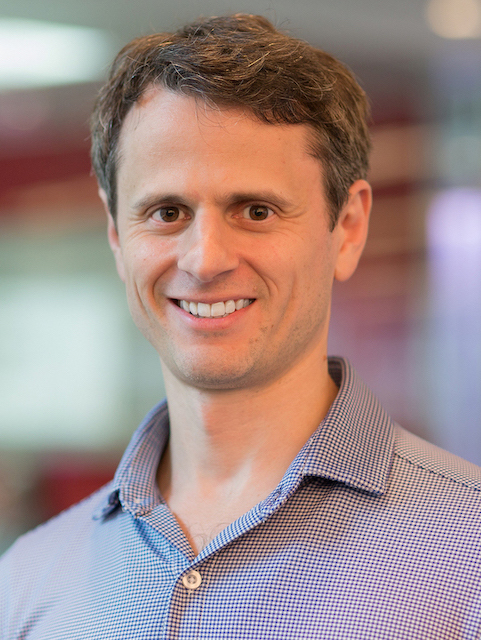
\includegraphics[width=\linewidth]{David_Rosenberg.jpg}
  \end{center}  
  \vspace{-25pt}
\end{wrapfigure}

\paragraph{Instructor}
Dr. David Rosenberg is a Data Scientist in the data science group in the
Office of the CTO at Bloomberg, and an Adjunct Associate Professor at
the Center for Data Science at New York University, where he has
repeatedly received NYU's Center for Data Science ``Professor of the
Year" award. He received his Ph.D. in statistics from UC Berkeley,
where he worked on statistical learning theory and natural language
processing. David received a Master of Science in applied mathematics,
with a focus on computer science, from Harvard University, and a
Bachelor of Science in mathematics from Yale University.


\paragraph{Outline}
There is no shortage of tutorials describing a huge variety of machine
learning models and techniques. In this short course, we take a step
back and present a coherent framework for thinking about supervised
machine learning models in general. We examine multiple examples of
the four fundamental components of a machine learning method: loss
function, regularization, hypothesis space, and optimization
method. Within this framework, we'll study linear regression
(regression, lasso, and elastic net) and classification methods. We'll
also introduce the most important nonlinear models, including
tree-based ensemble methods and neural network
models. Time-permitting, we may discuss conditional probability
models, noting that the vast majority of contemporary deep learning
models are of this type, as well as an approach to multiclass
classification that generalizes to structured prediction and ranking
problems, among many other applications. Throughout our discussion,
we'll introduce the terminology and notation used by experts in
machine learning to help bridge the gap between introductory-level
tutorials and the more advanced materials you can find at conferences
and in graduate-level courses.

\paragraph{Prerequisites}
Familiarity with basic mathematical notation (e.g., $\sum$ for summation,
$\arg\min$), basic linear algebra (e.g., matrix multiplication,
projections, inner products, norms, and spans), and introductory
probability (probability distributions, conditional probability and
conditional expectation).

\subsection*{\blue{Course 2 (Full Day): Big Data Analytics and Deep
  Learning}}

\begin{wrapfigure}{r}{3cm}
  \vspace{-25pt}
  \begin{center}
    
\includegraphics[width=\linewidth]{Hui-Lin.png}
  \end{center}  
  \vspace{-25pt}
\end{wrapfigure}
\paragraph{Instructors}
Dr. Hui Lin is leading and building data science department at
Netlify. Before Netlify, she was a Data Scientist at DuPont. She was a
leader in the company of applying advanced data science to enhance
Marketing and Sales Effectiveness. She provided data science
leadership for a broad range of predictive analytics and market
research analysis from 2013 to 2018. She is the co-founder of Central
Iowa R User Group, blogger of scientistcafe.com and 2018 Program Chair
of ASA Statistics in Marketing Section. She enjoys making analytics
accessible to a broad audience and teaches tutorials and workshops for
practitioners on data science. She holds MS and Ph.D in statistics
from Iowa State University.


\begin{wrapfigure}{r}{3cm}
  \vspace{-25pt}
  \begin{center}
    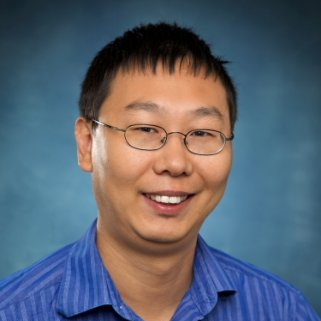
\includegraphics[width=\linewidth]{Ming-Li.png}
  \end{center}  
  \vspace{-25pt}
\end{wrapfigure}
Dr. Ming Li is currently a Research Scientist at Amazon.
He organized and presented 2018 JSM
Introductory Overview Lecture: Leading Data Science: Talent, Strategy,
and Impact. He was the Chair of Quality \& Productivity Section of ASA
for 2017. He was a Data Scientist at Walmart and a Statistical Leader
at General Electric Global Research Center. He obtained his Ph.D. in
Statistics from Iowa State University in 2010. With deep statistics
background and a few years’ experience in data science, he has trained
and mentored numerous junior data scientists with different background
such as statistician, programmer, software developer, database
administrator and business analyst. He is also an Instructor of
Amazon’s internal Machine Learning University and was one of the key
founding member of Walmart’s Analytics Rotational Program which
bridges the skill gaps between new hires and productive data
scientists.


\paragraph{Outline}

In the past couple of years, deep learning has gained traction in many
areas. It becomes an essential tool in data scientist’s toolbox. In
this course, students will develop a clear understanding of the big
data cloud platform, technical skills in data sciences and machine
learning, the motivation and use cases of deep learning through
hands-on exercises. We will also cover the ``art'' part of data
science: data science project flow, general pitfalls in data science
and machine learning, and soft skills to effectively communicate with
business stakeholders. The course is for audience with statistics
background. We use real-world data science and machine learning
problems to illustrate data science workflow, pitfalls, and soft
skills. The hands-on sessions use Databricks community edition cloud
platform. Specific modules are: 
(1) big data platform using Spark through R \pkg{sparklyr} package;
(2) introduction to deep neural network, convolutional neural network
recurrent neural networks, and their applications;
(3) deep learning examples using TensorFlow through R \pkg{keras}
package.


\paragraph{Prerequisites}

Introductory statistics or practical experience in data science ;
entry level of R knowledge; a free Databrick Community Edition account
through \url{https://databricks.com/try-databricks}; a laptop.


\subsection*{\blue{Course 3 (Half Day): Practical Visualization for Data Scientists}}


\begin{wrapfigure}{r}{3cm}
  \vspace{-25pt}
  \begin{center}
    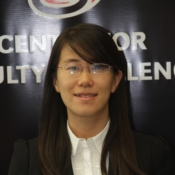
\includegraphics[width=\linewidth]{Cheng-Xiaoyue.jpg}
  \end{center}  
  \vspace{-25pt}
\end{wrapfigure}
\paragraph{Instructor}
Dr. Xiaoyue Cheng is an Assistant Professor in the Department of
Mathematics, University of Nebraska at Omaha. She received her
Ph.D. in Statistics from Iowa State University in 2015. Her research
interests include data visualization, interactive graphics, image
recognition, machine learning, statistical computing and simulation,
exploratory data analysis, and missing data analysis. She has
extensive interdisciplinary research experience in a variety of fields
including education, ethnicity population, psychology, medical
clinics, public health, engineering, aviation, agronomy, and business
marketing. Cheng is the main author of five R packages:
\pkg{MissingDataGUI}, \pkg{cranvas}, \pkg{cartogram},
\pkg{ePort}, and \pkg{MergeGUI}.


\paragraph{Outline}
Visualization has an important role in data science as it is widely
used for data exploration, information delivery, and communication
among people at different positions or from different
backgrounds. Specifically, statistical graphics focuses on revealing
the patterns, trends, and relationships from dataset with complex
challenges including the massive amount, high dimensions, and various
formats of data. This short course will introduce the advanced
programming skills to accurately and attractively communicate data
information with visualization. Topics of the course will include (1)
the elements and grammar of graphics via the \pkg{ggplot2} package;
(2) interactive web apps by the \pkg{shiny} package; (3) time series data
visualization using the \pkg{dygraphs} package; (4) geographic/map/GIS data
visualization using the \pkg{leaflet} package; and (5) interactive graphics with
the \pkg{plotly} package. Depending on the audience, example data from
different research topics such as the US Census Bureau, business
marketing, clinical trials, images, etc., will be applied to
demonstrate the visual methods. R language will be employed for this
course, and the attendees will have the chance to generate graphs on
their own for all of the topics.

\paragraph{Prerequisites}
Introductory statistics; basic programming experience with R; a laptop.

\subsection*{\blue{Course 4 (Half-Day): Introduction to Multilevel Modeling}}

\begin{wrapfigure}{r}{3cm}
  \vspace{-25pt}
  \begin{center}
    
\includegraphics[width=\linewidth]{Zhu-Min.jpg}
  \end{center}
  \vspace{-25pt}
\end{wrapfigure}
\paragraph{Instructor}
Dr. Min Zhu is a senior research statistician developer at SAS
Institute Inc. She joined SAS in 2009 after receiving her Ph.D in
Statistics from University of New Mexico. Her research and development
focus is the generalized linear mixed model procedure
(\textsf{PROC GLIMMIX}).
She works closely with statisticians and researchers in both
academia and industry on performance and functionality improvement in
\textsf{PROC GLIMMIX}.
Her recent work include enhancements for small sample
inference, efficient numerical integration, and multilevel weighting
for complex survey analysis. Dr. Zhu enjoys advocating the tool of
mixed models to the community of statisticians and data analysts. She
has organized sessions and taught courses on generalized linear mixed
models at Joint Statistical Meeting, SAS Global Forum, and ASA
Biopharmaceutical Section FDA-Industry Workshop.


\paragraph{Outline}
Hierarchical data are common in many fields, from pharmaceuticals to
agriculture to sociology. As you collect more and more data,
information is likely to be observed on nested units at multiple
levels, calling for a multilevel modeling approach. This course will
show you how to construct a multilevel model to account for
variability at each level through both explanatory and random
variables, in a way that shows the close relationship between
multilevel models and mixed models. You will learn how to use
generalized linear mixed models to estimate multilevel models for both
continuous and discrete responses. You will see examples that
illustrate the flexibility multilevel offers for modeling
within-cluster correlation, for disentangling multilevel explanatory
variables, and for differentiating between-cluster and within-cluster
effects. You will also learn about weighted multilevel models that
handle weights at different levels. Finally, you will see how to apply
weighted multilevel models to the analysis of complex survey data that
are collected by multistage sampling with unequal sampling
probabilities.

\paragraph{Prerequisites}
Introductory courses in statistical modeling and
statistical inference; experience with multilevel data.

\end{document}
